\documentclass[a4paper,12pt]{article}

% include headers and preamble for reoport
% file: includes-report.tex
% -----------------------------------------------------------------------------
% includes for studies report
% -----------------------------------------------------------------------------

\usepackage{amsmath}
\usepackage{setspace}
\usepackage[top=1.2in, bottom=1.2in]{geometry}
\usepackage[x11names]{xcolor}

\usepackage{float} % to force placement of images etc.

\usepackage{graphicx}
\usepackage[utf8]{inputenc}
\usepackage{siunitx}

% // -- for different section heading color --
\usepackage{sectsty}
\usepackage{xcolor}
% \chapterfont{\color{blue}}  % sets colour of chapters
% \definecolor{MyBlue}{rgb}{0.78,0.9,1} % rgb color code
% \definecolor{DarkBlue}{HTML}{002f4c} % HTML HEX color code
\definecolor{DarkBlue}{RGB}{0,47,76} % RGB color code
\sectionfont{\color{DarkBlue}}  % sets colour of sections
\subsectionfont{\color{DarkBlue}}  % sets colour of sections

\usepackage{float}


%\usepackage{multirow}
%\usepackage{pgfplots}
\usepackage{subcaption}

% // -- for source code listings --
\usepackage{color}
\definecolor{OliveGreen}{RGB}{0,128,0}
\usepackage{listings}
\usepackage{caption}
\DeclareCaptionFont{white}{\color{white}}
\DeclareCaptionFormat{listing}{\colorbox{gray}{\parbox{\textwidth}{#1#2#3}}}
\captionsetup[lstlisting]{format=listing,labelfont=white,textfont=white}


\lstdefinestyle{cStyle}{language=C}
\lstset{
language=C,
%basicstyle=\small\ttfamily,
basicstyle=\small\ttfamily,
keywordstyle=\color{blue}\ttfamily,
stringstyle=\color{red}\ttfamily,
commentstyle=\color{magenta}\ttfamily,
morecomment=[l][\color{magenta}]{\#},
numbers=left,
numberstyle=\tiny,
% frame=tb,
columns=fullflexible,
showstringspaces=false,
tabsize=2
}
\usepackage{matlab-prettifier}
\lstdefinestyle{matlabStyle}{language=matlab}
\lstset{
%style=Matlab-editor,
language=matlab,
%basicstyle=\small\ttfamily,
basicstyle=\small\ttfamily,
keywordstyle=\color{blue}\ttfamily,
stringstyle=\color{red}\ttfamily,
commentstyle=\color{OliveGreen}\ttfamily,
morecomment=[l][\color{OliveGreen}]{\#},
numbers=left,
numberstyle=\tiny,
% frame=tb,
columns=fullflexible,
showstringspaces=false,
tabsize=2
}
\lstdefinestyle{vhdlStyle}{language=vhdl}
\lstset{
language=vhdl,
%basicstyle=\small\ttfamily,
basicstyle=\small\ttfamily,
keywordstyle=\color{blue}\ttfamily,
stringstyle=\color{red}\ttfamily,
commentstyle=\color{magenta}\ttfamily,
morecomment=[l][\color{magenta}]{\#},
numbers=left,
numberstyle=\tiny,
% frame=tb,
columns=fullflexible,
showstringspaces=false,
tabsize=2
}

% bibliography (Literaturverzeinis)
\usepackage[round]{natbib}
\bibliographystyle{alphadin} % set format

% // -- source code listings --


\title{Bachelorprojekt}
\date{2018-11-21}
\author{Fabian Huber}

\begin{document}

% Titlepage for HAW lab report
\begin{titlepage}
\definecolor{blue(ncs)}{rgb}{0.0, 0.53, 0.74}
\begin{figure}[h!]
  \begin{flushright}
  \begin{spacing}{1.5}
  
\includegraphics[width=.5\linewidth]{images/hawlogo.png}
  \label{fig:hawlogo}\\
  \small Fakultät Technik und Informatik\\
  \small Department Informations- und Elektrotechnik
  \end{spacing}
  \end{flushright}
\end{figure}
\textbf{\large Bachelorprojekt}
\begin{center}\noindent\textcolor{blue(ncs)}{\rule{13.5cm}{0.5mm}}\end{center}
\begin{spacing}{4.5}
\textbf{\huge Automated Driving}
\end{spacing}
\textbf{\large\indent RC Car Control with Open Source Image Processing}
\begin{center}\noindent\textcolor{blue(ncs)}{\rule{13.5cm}{0.5mm}}\end{center}
\begin{spacing}{1.15}
\vspace*{\fill}
\noindent
\textnormal{\\
  Prof. Dr.-Ing. Marc Hensel \\
  \textbf{Projektgruppe:} Fabian Huber, Enzo Morino, Markus Trockel \\
  \textbf{Abgabe:} DD.MM.2019 \\
}
\end{spacing}
\end{titlepage}
% --- end of titlepage ---

  \pagenumbering{gobble}
  \newpage

  \tableofcontents
  \newpage

  \pagenumbering{arabic}

  \section{Einleitung}
    \ \\

  \section{Ziel des Projekts}
    \ \\
  
  \section{Kurzübersicht}
    \ \\

  \section{Hardware}
    \ \\
    \subsection{Raspberry Pi 3}
    \ \\
    \subsection{Motorcontroller}
    \ \\
    \subsection{Ultraschallsensor}
    \ \\
    \subsection{RC Fahrzeug}
    \ \\
  
  \section{Software}
    \ \\
    \subsection{Aufbau}
    \ \\
    \begin{minipage}{\columnwidth}
      \makeatletter
      \def\@captype{figure}
      \makeatother
      \centering
      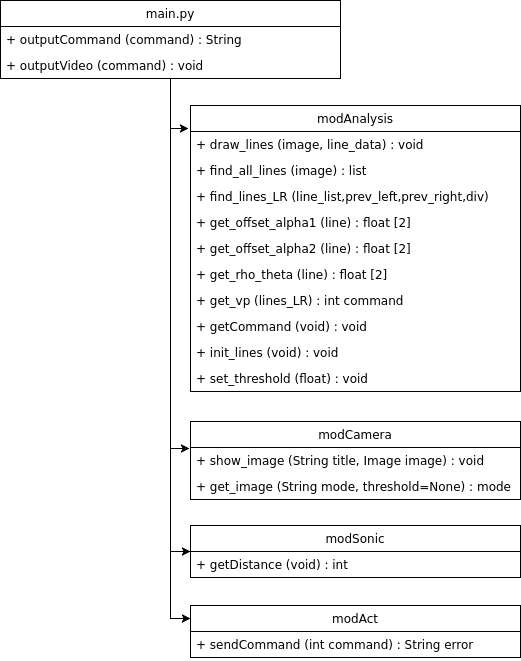
\includegraphics[width=0.8\linewidth]{images/code-flowchart.png}
      \caption{Aufbau des Python Codes}
      \label{fig:image-01}
    \end{minipage}
    \ \\

    \subsection{Externe Module}
    \ \\
    \begin{minipage}{\columnwidth}
      \makeatletter
      \def\@captype{table}
      \makeatother
      \centering
      %\rowcolors{1}{grey}{white}
      \begin{tabular}{ l | l }
      % \multicolumn{2}{|c}{Frame \#} & \multicolumn{4}{|c}{LCD 0/3} &
      Name & Beschreibung \\ \hline \hline
      tkinter & ... \\
      Adafruit\_PCA9685 & Bibliothek zur Ansteuerung des Motorcontrollers \\
      numpy & Bibliothek zur Verwendung von Matlab Funktionen \\
      cv2 & OpenCV 2 bietet Algorithmen zur Bildverarbeitung \\
      io & ... \\
      time & ... \\
      importlib & ... \\
      argparse & ... \\
      pivideostream & ... \\
      picamera & ... \\
      threading & ... \\
      RPi.GPIO & Bibliothek zur Ansteuerung der GPIO ports des Raspbery Pi \\
      \end{tabular}
      \caption{verwendete externe Python Module}
      \label{tab:01}
    \end{minipage}
    
    \subsection{Eigene Module}
    \ \\
    \begin{minipage}{\columnwidth}
      \makeatletter
      \def\@captype{table}
      \makeatother
      \centering
      %\rowcolors{1}{grey}{white}
      \begin{tabular}{ l | l }
      % \multicolumn{2}{|c}{Frame \#} & \multicolumn{4}{|c}{LCD 0/3} &
      Name & Beschreibung \\ \hline \hline
      modAnalysis & Verantwortlich für die eigentliche Verarbeitung der visuellen Informationen \\
      modAct & Verantwortlich für die Ansteuerung des Motors und der Lenkung \\
      modCamera & Bereitet das Kamerabild für die Verarbeitung und Anzeige vor. \\
      modSonic & Kommuniziert mit dem Ultraschallsensor und liefert Distanz zum Hindernis.\\
      \end{tabular}
      \caption{verwendete eigene Python Module}
      \label{tab:01}
    \end{minipage}

  % \bibliography{hawey-documentation}
  % \bibliographystyle{ieeetr}

\end{document}
